%!TEX program = xelatex

\documentclass[compress]{beamer}
%--------------------------------------------------------------------------
% Common packages
%--------------------------------------------------------------------------
\usepackage[english]{babel}
\usepackage{pgfpages} % required for notes on second screen
\usepackage{graphicx}

\usepackage{multicol}

\usepackage{tabularx,ragged2e}
\usepackage{booktabs}

\usepackage{listings}
\lstset{ %
language=[LaTeX]TeX,
basicstyle=\normalsize\ttfamily,
keywordstyle=,
numbers=left,
numberstyle=\tiny\ttfamily,
stepnumber=1,
showspaces=false,
showstringspaces=false,
showtabs=false,
breaklines=true,
frame=tb,
framerule=0.5pt,
tabsize=4,
framexleftmargin=0.5em,
framexrightmargin=0.5em,
xleftmargin=0.5em,
xrightmargin=0.5em
}


%--------------------------------------------------------------------------
% Load theme
%--------------------------------------------------------------------------
\usetheme{hri}

\usepackage{dtklogos} % must be loaded after theme
\usepackage{tikz}
\usetikzlibrary{intersections,arrows,shapes,calc,mindmap,backgrounds,positioning,svg.path}

\graphicspath{{figs/}}

%--------------------------------------------------------------------------
% General presentation settings
%--------------------------------------------------------------------------
\title{The Robot Operating System}
\subtitle{High-Altitude Overview of ROS}
\date{\today}
\author{Séverin Lemaignan}
\institute{Centre for Robotics and Neural Systems\\ {\Medium Plymouth University}}

%--------------------------------------------------------------------------
% Notes settings
%--------------------------------------------------------------------------
%\setbeameroption{show notes on second screen}

\begin{document}
%--------------------------------------------------------------------------
% Titlepage
%--------------------------------------------------------------------------

\maketitle

%--------------------------------------------------------------------------
% Table of contents
%--------------------------------------------------------------------------
%\section*{Overview}
%\begin{frame}{Overview}
%	% hideallsubsections ist empfehlenswert für längere Präsentationen
%	\tableofcontents[hideallsubsections]
%\end{frame}

%--------------------------------------------------------------------------
% Content
%--------------------------------------------------------------------------
\section{ROS is not an operating system}

\begin{frame}{Instead, ROS is...}
    \begin{itemize}
        \item<1-> A fairly simple message passing system designed with robotics in
            mind
        \item<2-> An API to this system (in several languages -- C++ and Python are
            1st tier)
        \item<3-> A set of standard message types that facilitate interoperability between modules
        \item<4> \Medium{A middleware?}
        \item<5-> A set of conventions to write and package robotic softwares
        \item<6-> Deep integration of a few key open-source libraries (OpenCV, PCL, tf)
        \item<7-> A set of tools to run and monitor the nodes
        \item<8-> Engagement of a large academic community, leading to a library of thousands of nodes
    \end{itemize}
\end{frame}

\begin{frame}{ROS Ecosystem}
    \centering
    \resizebox{0.9\textwidth}{!}{%
        \vspace*{4cm}
        \begin{tikzpicture}

            \path[small mindmap,
                  level 1 concept/.append style={sibling angle=360/5}, 
                  level 2 concept/.append style={sibling angle=60}, 
                  concept color=hriWarmGreyLight,text=hriWarmGreyDark]

            node[concept] {\Medium ROS}
            [clockwise from=-180]
            child[concept color=hriSec1Dark,text=white] { node[concept]{Middleware} 
                [clockwise from=-120]
                child[concept color=hriSec1CompDark,text=white] { node[concept]{Standard Interfaces} }
                child[concept color=hriSec3CompDark,text=white] { node[concept]{Nodes Management} }
                child[concept color=hriSec2Dark,text=white] { node[concept]{IPC} }
            }
            child[concept color=hriSec3Comp,text=white] { node[concept] {Standards and Conventions} }
            child[concept color=hriSec2CompDark,text=white] { node[concept]{Community}
                [clockwise from=90]
                child[concept color=hriSec2Comp,text=white] { node[concept]{Software engineering infrastructure} }
                child[concept color=hriSec1,text=white] { node[concept] {REPs} }
                child[concept color=hriSec3,text=white] { node[concept] {ROSCon} }
            }
            child[concept color=hriSec3Dark,text=white] { node[concept] {Large software library} 
                [clockwise from=0]
                child[concept color=hriSec2Dark,text=white] { node[concept] {Satellite libraries} }
            }
            child[concept color=hriSec3CompDark,text=white] { node[concept] {Tooling} };
        \end{tikzpicture}
    }
\end{frame}

\begin{frame}{}
    This being clarified...
\end{frame}

\section{How does it look like?}

\begin{frame}[containsverbatim]{}

\begin{shcode}
$ roscore
$ rosrun rviz rviz
$ roslaunch openni_launch openni.launch
\end{shcode}

\end{frame}


\imageframe{rviz0}

\begin{frame}[containsverbatim]{}

\begin{shcode}
$ rosrun attention_tracker estimate 
                         image:=/camera/rgb/image_color
\end{shcode}

\end{frame}

\imageframe{rviz}

\begin{frame}[containsverbatim]{}
\begin{shcode}
$ rosnode list 
/camera_base_link
/camera_base_link1
/camera_base_link2
/camera_base_link3
/ros_attention_tracker
/rosout
/camera/camera_nodelet_manager
/camera/debayer
/camera/depth_metric
/camera/depth_metric_rect
/camera/depth_points
/camera/depth_rectify_depth
/camera/depth_registered_hw_metric_rect
/camera/depth_registered_metric
/camera/depth_registered_rectify_depth
/camera/depth_registered_sw_metric_rect
/camera/disparity_depth
/camera/disparity_registered_hw
/camera/disparity_registered_sw
/camera/driver
/camera/points_xyzrgb_hw_registered
/camera/points_xyzrgb_sw_registered
/camera/rectify_color
/camera/rectify_ir
/camera/rectify_mono
/camera/register_depth_rgb
\end{shcode}

\end{frame}

\begin{frame}[containsverbatim]{}
\begin{shcode}
$ rostopic list
/camera_info
/image
/nb_detected_faces
/rosout
/rosout_agg
/tf
/camera/depth/image_rect_raw
/camera/depth/image_rect_raw/compressed
/camera/depth/image_rect_raw/compressed/parameter_descriptions
/camera/depth/image_rect_raw/compressed/parameter_updates
/camera/depth/image_rect_raw/compressedDepth
/camera/depth/image_rect_raw/compressedDepth/parameter_descriptions
/camera/depth/image_rect_raw/compressedDepth/parameter_updates
/camera/depth/image_rect_raw/theora
/camera/depth/image_rect_raw/theora/parameter_descriptions
/camera/depth/image_rect_raw/theora/parameter_updates
/camera/depth_rectify_depth/parameter_descriptions
/camera/depth_rectify_depth/parameter_updates
\end{shcode}

\end{frame}

\begin{frame}[containsverbatim]{}
\begin{shcode}
$ rostopic echo tf
transforms: 
  - 
    header: 
      seq: 0
      stamp: 
        secs: 1449222890
        nsecs: 396561780
      frame_id: /camera_link
    child_frame_id: /camera_rgb_frame
    transform: 
      translation: 
        x: 0.0
        y: -0.045
        z: 0.0
      rotation: 
        x: 0.0
        y: 0.0
        z: 0.0
        w: 1.0
---
transforms: 
  - 
    header: 
      seq: 0
      stamp: 
        secs: 1449222890

\end{shcode}

\end{frame}


\begin{frame}[containsverbatim]{}

\begin{shcode}
$ rosrun rqt_reconfigure rqt_reconfigure
\end{shcode}

\end{frame}


\imageframe{dynamic_reconfigure.png}

\begin{frame}{Example: a simple image processing pipeline}

\begin{center}
\begin{tikzpicture}[
                    >=latex,
                    every edge/.style={->, draw, very thick},
                    service/.style={->, draw, very thick,dashed},
                    rosnode/.style={draw, font=\sf, node distance=0.5, rounded
                    corners, align=center, inner sep=5pt,fill=hriSec2Dark!50},
                    topic/.style={font=\tt, node distance=0.5, align=center, inner sep=5pt},
                    pic/.style={fill=none,draw=none}
                ]

    \node [rosnode] at (-4,0) (node1) {image acquisition};
    \node [rosnode] at (0,-2) (node2) {image processor};
    \node [rosnode] at (4,-4) (node3) {next processing};

        \node [topic] at (-4,-1.5) (topic3) {/image};
        \node [topic] at (-1,-3.5) (topic1) {/processed\_image};
        \path (node1) edge[bend right] (node2);
        \path (node2) edge[bend right] (node3);


\end{tikzpicture}
\end{center}

\end{frame}

%\begin{frame}{Example: a simple image processing pipeline}
%
%\begin{center}
%\begin{tikzpicture}[
%                    >=latex,
%                    every edge/.style={->, draw, very thick},
%                    service/.style={->, draw, very thick,dashed},
%                    rosnode/.style={draw, font=\sf, node distance=0.5, rounded
%                    corners, align=center, inner sep=5pt,fill=hriSec2Dark!50},
%                    topic/.style={font=\tt, node distance=0.5, align=center, inner sep=5pt},
%                    pic/.style={fill=none,draw=none}
%                ]
%
%    \node [rosnode] at (-4,0) (node1) {\tt gscam};
%    \node [rosnode] at (0,-2) (node2) {\tt our\_processing};
%    \node [rosnode] at (4,-4) (node3) {\tt next\_processing};
%
%        \node [topic] at (-1.2,-0.7) (topic2) {/v4l/camera/image\_raw};
%        \node [topic] at (-2.4,-2.2) (topic3) {/image};
%        \node [topic] at (1.4,-2.7) (topic1) {/processed\_image};
%        \path (node1) edge[bend right] (node2);
%        \path (node2) edge[bend right] (node3);
%
%
%\end{tikzpicture}
%\end{center}
%
%\end{frame}


\begin{frame}[containsverbatim]{}

\begin{pythoncode}
import sys, cv2, rospy
from sensor_msgs.msg import Image
from cv_bridge import CvBridge

def on_image(image):
    cv_image = bridge.imgmsg_to_cv2(image, "bgr8")
    (rows,cols,channels) = cv_image.shape
    cv2.circle(cv_image, (cols/2,rows/2), 50,(0,0,255), -1)
    cv2.imshow("Image window", cv_image)
    cv2.waitKey(3)
    image_pub.publish(bridge.cv2_to_imgmsg(cv_image, "bgr8"))

rospy.init_node('image_processor')
bridge = CvBridge()
image_sub = rospy.Subscriber("image",Image, on_image)
image_pub = rospy.Publisher("processed_image",Image)

while not rospy.is_shutdown():
    rospy.spin()
\end{pythoncode}

\end{frame}

\begin{frame}[containsverbatim]{}

\begin{shcode}
$ roslaunch gscam v4l.launch
$ python image_processor.py image:=/v4l/camera/image_raw
$ rosrun image_view image_view image:=/processed_image
\end{shcode}

\end{frame}


\imageframe{image_processor.png}




\section{Into the details: the key concepts}

\begin{frame}{Talking Nodes}

\begin{center}
\begin{tikzpicture}[
                    >=latex,
                    every edge/.style={->, draw, very thick},
                    service/.style={->, draw, very thick,dashed},
                    rosnode/.style={draw, font=\sf, node distance=0.5, rounded
                    corners, align=center, inner sep=5pt,fill=hriSec2Dark!50},
                    topic/.style={font=\tt, node distance=0.5, align=center, inner sep=5pt},
                    pic/.style={fill=none,draw=none}
                ]

    \path[use as bounding box] (-6,1) rectangle (6,-5);
    \node [rosnode] at (0,0) (node1) {node 1};
    \node [rosnode] at (4,-2) (node2) {node 2};
    \node [rosnode] at (-5,-4) (node3) {node 3};

    \uncover<2-> {
        \node [topic] at (1,-2) (topic1) {/topic1};
        \node [topic] at (-1,-3) (topic2) {/topic2};
        \node [topic] at (-4,-2) (topic3) {/topic3};
        \path (node1) edge[bend left] node[label,right] {\only<2-3>{publishes}} (topic1);
        \path (node1) edge[bend right] node[label,left] {\only<2-3>{publishes}} (topic2);
        \path (node3) edge[bend left] node[label,left] {\only<2-3>{publishes}} (topic3);
    }
    \uncover<3-> {
        \path (topic1) edge[bend right] node[label,below left] {\only<3>{subscribes}} (node2);
        \path (topic2) edge[bend left] node[label,below] {\only<3>{subscribes}} (node3);
        \path (topic2) edge[bend right] (node2);
    }
    \only<4-5> {
        \path[->, dashed] ([yshift=2pt]node1.east) edge[bend left] node[label,above right] {service (RPC)} ([xshift=2pt]node2.north) ;
    }
    \only<5> {
        \path[->, dashed] ([xshift=-2pt]node2.north) edge[bend right] ([yshift=-2pt]node1.east);

    }

    \uncover<6-> {
        \path[->, dashed] ([yshift=2pt]node1.east) edge[bend left] node[label,above right] {action goal} ([xshift=2pt]node2.north) ;
    }
    \uncover<7-> {
        \path[->, dashed] ([xshift=-2pt]node2.north) edge[bend right] node[label,below left] {result} ([yshift=-2pt]node1.east);

    }


\end{tikzpicture}
\only<5>{Services: \Medium synchronous}
\only<7>{Actions: \Medium asynchronous}
\end{center}

\end{frame}

\begin{frame}[containsverbatim]{Messages}

\begin{shcode}
$ rosmsg show geometry_msgs/Pose
geometry_msgs/Point position
  float64 x
  float64 y
  float64 z
geometry_msgs/Quaternion orientation
  float64 x
  float64 y
  float64 z
  float64 w
\end{shcode}
\end{frame}

\begin{frame}[containsverbatim]{Messages}
\begin{shcode}
$ rosmsg show sensor_msgs/Image 
std_msgs/Header header
    uint32 seq
    time stamp
    string frame_id
uint32 height
uint32 width
string encoding
uint8 is_bigendian
uint32 step
uint8[] data
\end{shcode}

\end{frame}

\begin{frame}[containsverbatim]{Messages}
\begin{shcode}
$ rostopic echo /camera/image_raw 
header: 
    seq: 56
    stamp: 
      secs: 1449243166
      nsecs: 415330019
    frame_id: /camera_frame
height: 720
width: 1280
encoding: rgb8
is_bigendian: 0
step: 3840
data: [32, 57, 51, 36, 61, 55, 41, 63, 60,...
\end{shcode}
\end{frame}


\begin{frame}{ROS vs YARP terminology}
    \begin{table}[]
        \begin{tabularx}{\linewidth}{l>{\raggedright}X}
            \toprule
            \textbf{YARP}			& \textbf{ROS} \tabularnewline
            \midrule
            \texttt{Port}		& \texttt{topic} \tabularnewline
            \texttt{RpcClient/RpcServer} & \texttt{action} (async) or \texttt{service} (sync) \tabularnewline
            \texttt{Bottle}		& \texttt{message} \tabularnewline
            \bottomrule
        \end{tabularx}
        \label{tab:options}
    \end{table}

    Connections of ports: explicit with YARP, implicit with ROS
\end{frame}


\begin{frame}{Transformations}
    \only<1>{
    \begin{center}
        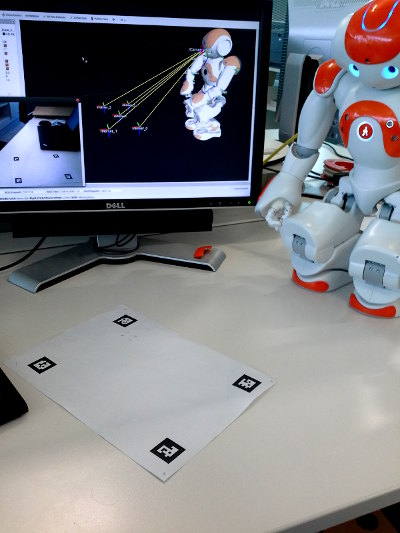
\includegraphics[height=0.9\textheight]{nao_markers}
    \end{center}
}
%\only<2> {
%    % Sketch output, version 0.3 (build 7d, Wed May 2 06:36:52 2012)
% Output language: PGF/TikZ,LaTeX
\begin{tikzpicture}[line join=round]
\filldraw[box](-3.055,1.164)--(-3.293,1.104)--(-3.323,1.532)--(-3.081,1.579)--cycle;
\filldraw[box](-3.055,1.164)--(-2.691,1.144)--(-2.715,1.564)--(-3.081,1.579)--cycle;
\filldraw[box](-3.055,1.164)--(-2.691,1.144)--(-2.92,1.083)--(-3.293,1.104)--cycle;
\filldraw[box](-3.081,1.579)--(-3.323,1.532)--(-2.947,1.516)--(-2.715,1.564)--cycle;
\filldraw[box](-2.691,1.144)--(-2.715,1.564)--(-2.947,1.516)--(-2.92,1.083)--cycle;
\filldraw[box](-3.323,1.532)--(-3.293,1.104)--(-2.92,1.083)--(-2.947,1.516)--cycle;
\filldraw[box](1.983,2.444)--(2.385,2.423)--(1.92,2.409)--(1.527,2.431)--cycle;
\filldraw[box](1.983,2.444)--(2.385,2.423)--(2.416,3.048)--(2.007,3.044)--cycle;
\filldraw[box](1.983,2.444)--(1.527,2.431)--(1.546,3.047)--(2.007,3.044)--cycle;
\filldraw[box](-.16,1.439)--(-.674,1.399)--(-.683,2.005)--(-.162,2.029)--cycle;
\filldraw[box](-.16,1.439)--(.152,1.374)--(.154,1.989)--(-.162,2.029)--cycle;
\filldraw[box](-.16,1.439)--(.152,1.374)--(-.377,1.331)--(-.674,1.399)--cycle;
\filldraw[box](2.007,3.044)--(1.546,3.047)--(1.945,3.051)--(2.416,3.048)--cycle;
\filldraw[box](-.162,2.029)--(-.683,2.005)--(-.382,1.963)--(.154,1.989)--cycle;
\filldraw[box](1.546,3.047)--(1.527,2.431)--(1.92,2.409)--(1.945,3.051)--cycle;
\filldraw[box](-.683,2.005)--(-.674,1.399)--(-.377,1.331)--(-.382,1.963)--cycle;
\filldraw[box](2.385,2.423)--(2.416,3.048)--(1.945,3.051)--(1.92,2.409)--cycle;
\filldraw[box](.152,1.374)--(.154,1.989)--(-.382,1.963)--(-.377,1.331)--cycle;
\filldraw[box](-1.341,-.884)--(-1.624,-1.086)--(-1.647,-.443)--(-1.359,-.271)--cycle;
\filldraw[box](-1.341,-.884)--(-.75,-.949)--(-.76,-.326)--(-1.359,-.271)--cycle;
\filldraw[box](-1.341,-.884)--(-.75,-.949)--(-1.006,-1.159)--(-1.624,-1.086)--cycle;
\filldraw[box](-1.359,-.271)--(-1.647,-.443)--(-1.021,-.505)--(-.76,-.326)--cycle;
\filldraw[box](-.75,-.949)--(-.76,-.326)--(-1.021,-.505)--(-1.006,-1.159)--cycle;
\filldraw[box](-1.647,-.443)--(-1.624,-1.086)--(-1.006,-1.159)--(-1.021,-.505)--cycle;
\filldraw[box](1.462,.372)--(1.913,.032)--(1.357,-.313)--(.919,.048)--cycle;
\filldraw[box](1.462,.372)--(1.913,.032)--(1.878,.57)--(1.409,.903)--cycle;
\filldraw[box](1.462,.372)--(.919,.048)--(.842,.575)--(1.409,.903)--cycle;
\filldraw[box](.842,.575)--(.919,.048)--(1.357,-.313)--(1.296,.221)--cycle;
\filldraw[box](1.913,.032)--(1.878,.57)--(1.296,.221)--(1.357,-.313)--cycle;
\filldraw[box](1.409,.903)--(.842,.575)--(1.296,.221)--(1.878,.57)--cycle;
\end{tikzpicture}% End sketch output

%}
\only<2> {
    \begin{center}
    % Sketch output, version 0.3 (build 7d, Wed May 2 06:36:52 2012)
% Output language: PGF/TikZ,LaTeX
\begin{tikzpicture}[line join=round]
\draw[dashed](-1.571,-1.156)--(-3.136,.897);
\draw[axis,color=red,arrows=->](-3.136,.897)--(-3.529,.784);
\draw[axis,color=blue,arrows=->](-3.136,.897)--(-3.18,1.56);
\draw[axis,color=green,arrows=->](-3.136,.897)--(-2.553,.861);
\node at (-2.434,.854) {\tiny y};\node at (-3.189,1.695) {\tiny z};\node at (-3.613,.76) {\tiny x};\filldraw[box](-3.055,1.164)--(-2.691,1.144)--(-2.92,1.083)--(-3.293,1.104)--cycle;
\filldraw[box](-3.055,1.164)--(-2.691,1.144)--(-2.715,1.564)--(-3.081,1.579)--cycle;
\filldraw[box](-3.055,1.164)--(-3.293,1.104)--(-3.323,1.532)--(-3.081,1.579)--cycle;
\filldraw[box](-3.081,1.579)--(-3.323,1.532)--(-2.947,1.516)--(-2.715,1.564)--cycle;
\filldraw[box](-2.691,1.144)--(-2.715,1.564)--(-2.947,1.516)--(-2.92,1.083)--cycle;
\filldraw[box](-3.323,1.532)--(-3.293,1.104)--(-2.92,1.083)--(-2.947,1.516)--cycle;
\draw[axis,color=green,arrows=->](2.01,2.007)--(2.656,1.942);
\draw[dashed](0,1.061)--(2.01,2.007);
\draw[axis,color=red,arrows=->](2.01,2.007)--(1.287,1.968);
\draw[axis,color=blue,arrows=->](2.01,2.007)--(2.049,2.943);
\draw[dashed](-1.571,-1.156)--(0,1.061);
\draw[axis,color=red,arrows=->](0,1.061)--(-.809,.983);
\draw[axis,color=blue,arrows=->](0,1.061)--(0,1.984);
\draw[axis,color=green,arrows=->](0,1.061)--(.511,.931);
\draw[dashed](0,1.061)--(1.577,.478);
\filldraw[box](1.983,2.444)--(2.385,2.423)--(1.92,2.409)--(1.527,2.431)--cycle;
\filldraw[box](1.983,2.444)--(2.385,2.423)--(2.416,3.048)--(2.007,3.044)--cycle;
\filldraw[box](1.983,2.444)--(1.527,2.431)--(1.546,3.047)--(2.007,3.044)--cycle;
\filldraw[box](-.16,1.439)--(-.674,1.399)--(-.683,2.005)--(-.162,2.029)--cycle;
\filldraw[box](-.16,1.439)--(.152,1.374)--(.154,1.989)--(-.162,2.029)--cycle;
\filldraw[box](-.16,1.439)--(.152,1.374)--(-.377,1.331)--(-.674,1.399)--cycle;
\filldraw[box](2.007,3.044)--(1.546,3.047)--(1.945,3.051)--(2.416,3.048)--cycle;
\node at (2.796,1.928) {\tiny y};\node at (2.057,3.135) {\tiny z};\node at (1.135,1.96) {\tiny x};\filldraw[box](-.162,2.029)--(-.683,2.005)--(-.382,1.963)--(.154,1.989)--cycle;
\node at (.621,.903) {\tiny y};\node at (0,2.173) {\tiny z};\node at (-.979,.967) {\tiny x};\filldraw[box](1.546,3.047)--(1.527,2.431)--(1.92,2.409)--(1.945,3.051)--cycle;
\draw[axis,color=red,arrows=->](-1.571,-1.156)--(-2.045,-1.505);
\draw[axis,color=blue,arrows=->](-1.571,-1.156)--(-1.604,-.197);
\draw[axis,color=green,arrows=->](-1.571,-1.156)--(-.645,-1.266);
\filldraw[box](-.683,2.005)--(-.674,1.399)--(-.377,1.331)--(-.382,1.963)--cycle;
\filldraw[box](2.385,2.423)--(2.416,3.048)--(1.945,3.051)--(1.92,2.409)--cycle;
\filldraw[box](.152,1.374)--(.154,1.989)--(-.382,1.963)--(-.377,1.331)--cycle;
\node at (-.454,-1.289) {\tiny y};\node at (-1.611,0) {\tiny z};\node at (-2.15,-1.582) {\tiny x};\draw[axis,color=green,arrows=->](1.577,.478)--(2.296,-.053);
\draw[axis,color=blue,arrows=->](1.577,.478)--(1.502,1.32);
\draw[axis,color=red,arrows=->](1.577,.478)--(.734,-.024);
\node at (2.451,-.167) {\tiny y};\node at (1.485,1.502) {\tiny z};\node at (.56,-.128) {\tiny x};\filldraw[box](1.462,.372)--(1.913,.032)--(1.357,-.313)--(.919,.048)--cycle;
\filldraw[box](1.462,.372)--(1.913,.032)--(1.878,.57)--(1.409,.903)--cycle;
\filldraw[box](1.462,.372)--(.919,.048)--(.842,.575)--(1.409,.903)--cycle;
\filldraw[box](.842,.575)--(.919,.048)--(1.357,-.313)--(1.296,.221)--cycle;
\filldraw[box](1.913,.032)--(1.878,.57)--(1.296,.221)--(1.357,-.313)--cycle;
\filldraw[box](1.409,.903)--(.842,.575)--(1.296,.221)--(1.878,.57)--cycle;
\node at (-1.554,-1.62) {\small\tt /map};\node at (-3.114,.573) {\small\tt /table};\node at (-.229,.686) {\small\tt /base\_link};\node at (2.64,1.65) {\small\tt /camera};\node at (2.41,.421) {\small\tt /hand};\end{tikzpicture}% End sketch output

    \end{center}
}
\end{frame}

\section{Tooling}

\begin{frame}{Tools}
    \begin{table}[]
        \begin{tabularx}{\linewidth}{l>{\raggedright}X}
            \toprule
            \texttt{rviz} & versatile 2D/3D visualization \tabularnewline
            \texttt{rosconsole} & Centralized logging \tabularnewline
            \texttt{rosbag} & Record and replay messages \tabularnewline
            \texttt{rqt\_reconfigure} & Live configuration of nodes \tabularnewline
            \texttt{rqt\_diagnostics} & Standardized diagnostics \tabularnewline
            \texttt{rosgraph} & plots the node network \tabularnewline
            + tons of introspection tools & Print out/publish/call messages, services, nodes \tabularnewline
            \bottomrule
        \end{tabularx}
        \label{tab:options}
    \end{table}
\end{frame}

\begin{frame}{ROS vs YARP terminology}
    \begin{table}[]
        \begin{tabularx}{\linewidth}{l>{\raggedright}X}
            \toprule
            \textbf{YARP}			& \textbf{ROS} \tabularnewline
            \midrule
            \texttt{yarpserver}		& \texttt{roscore} \tabularnewline
            \texttt{yarpscope/yarpview}		& \texttt{rviz} \tabularnewline
            \texttt{yarpdatadumper/yarpdataplayer}		& \texttt{rosbag} \tabularnewline
            \texttt{yarpmanager}		& \texttt{roslaunch} \tabularnewline
            \bottomrule
        \end{tabularx}
        \label{tab:options}
    \end{table}

\end{frame}

\imageframe{rviz}

\end{document}






